\documentclass[draft,linenumbers]{agujournal}
\draftfalse
\usepackage{hyperref}

\hypersetup{
    colorlinks=true,
    linkcolor=blue,
    filecolor=magenta,      
    urlcolor=cyan,
}

\journalname{Journal of Advances in Modeling Earth Systems (JAMES)}
\begin{document}
 \begin{figure}[h]
     \centering
     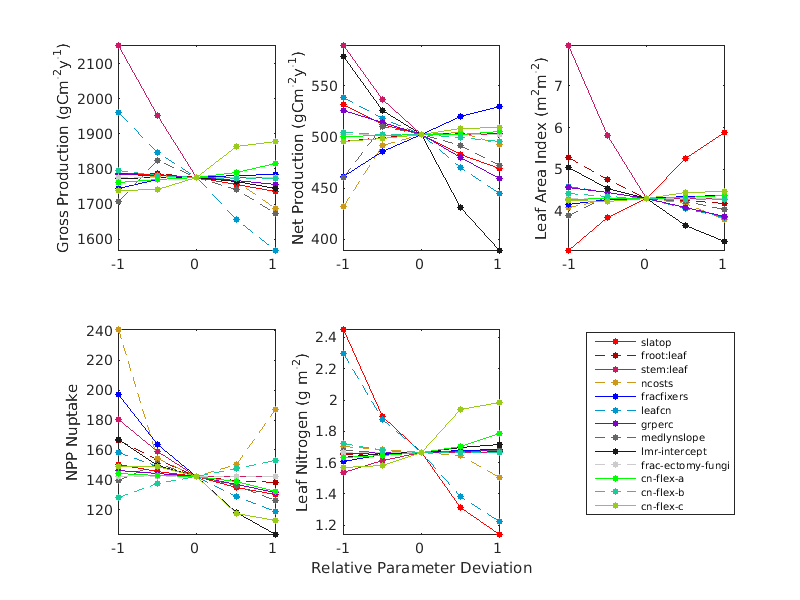
\includegraphics[width=35pc]{matlab/figures/frac_deviation_p1CLM5_CAX__y1.png}
     \caption{Caxiuana State Parameter Sensitivity}
     \label{CAX state}
  \end{figure}
  
   \begin{figure}[h]
     \centering
     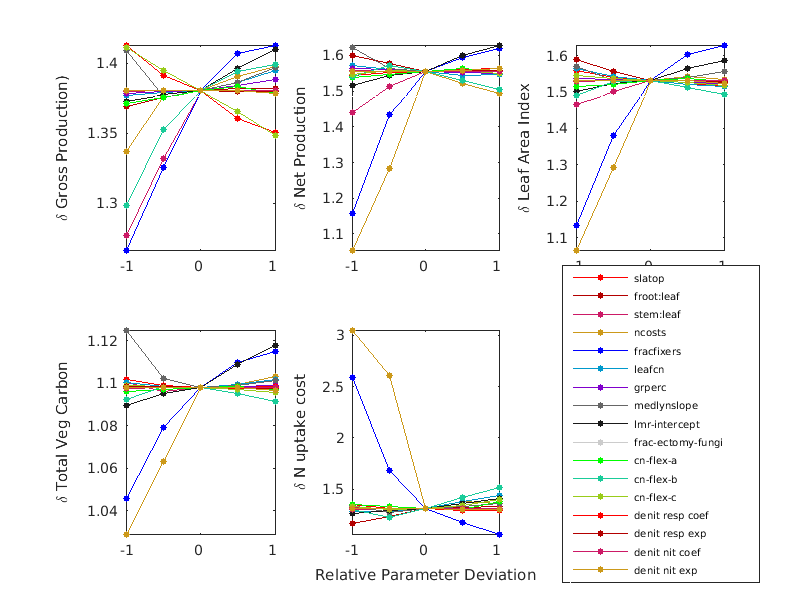
\includegraphics[width=35pc]{matlab/figures/frac_deviation_p1CLM5_BCI__y1.png}
     \caption{BCI State Parameter Sensitivity}
     \label{BCI state}
  \end{figure}
  
 \begin{figure}[h]
     \centering
     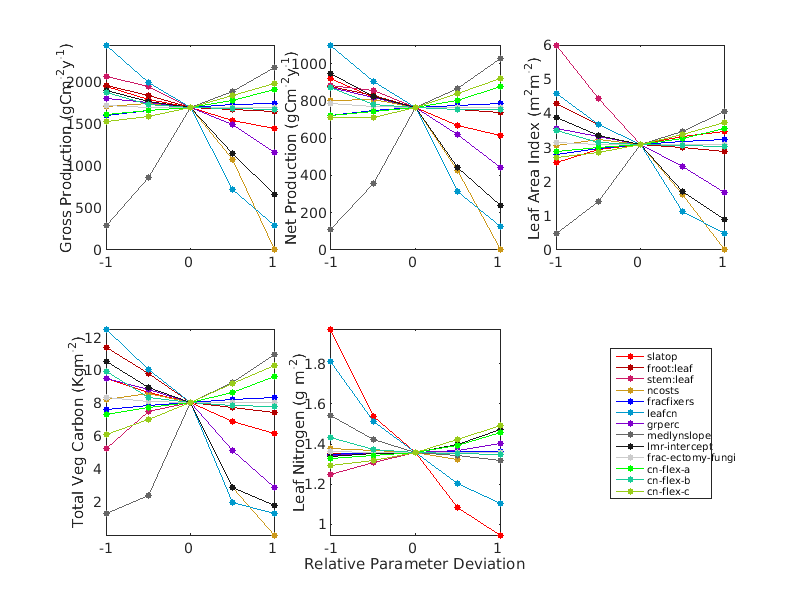
\includegraphics[width=35pc]{matlab/figures/frac_deviation_p1CLM5_ORN__y1.png}
     \caption{Oak Ridge State Parameter Sensitivity}
     \label{ORN state}
  \end{figure}
  
 \begin{figure}[h]
     \centering
     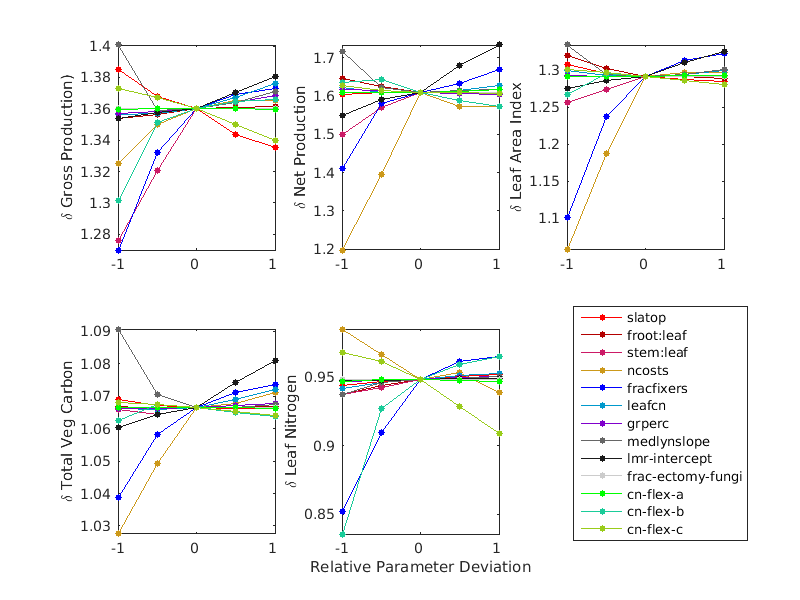
\includegraphics[width=35pc]{matlab/figures/frac_deviation_CO2_response_1CLM5_1x1pt_Br-cax_ens_transient_ELEV_PI_y1.png}
     \caption{Response to Nitrogen Deposition}
     \label{Caxiuana CO2 response Parameter Sensitivity }
  \end{figure}
  
  
  
 \begin{figure}[h]
     \centering
     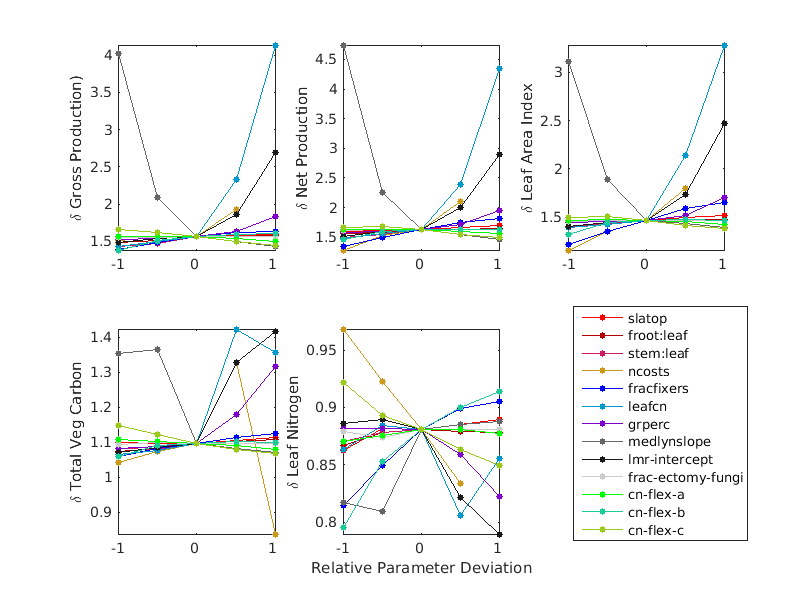
\includegraphics[width=35pc]{matlab/figures/frac_deviation_CO2_response_1CLM5_1x1pt_US-ORN_ens_transient_ELEV_PI_y1.png}
     \caption{Response to Nitrogen Deposition}
     \label{Oak Ridge CO2 response Parameter Sensitivity}
  \end{figure}
  
  
 \begin{figure}[h]
     \centering
     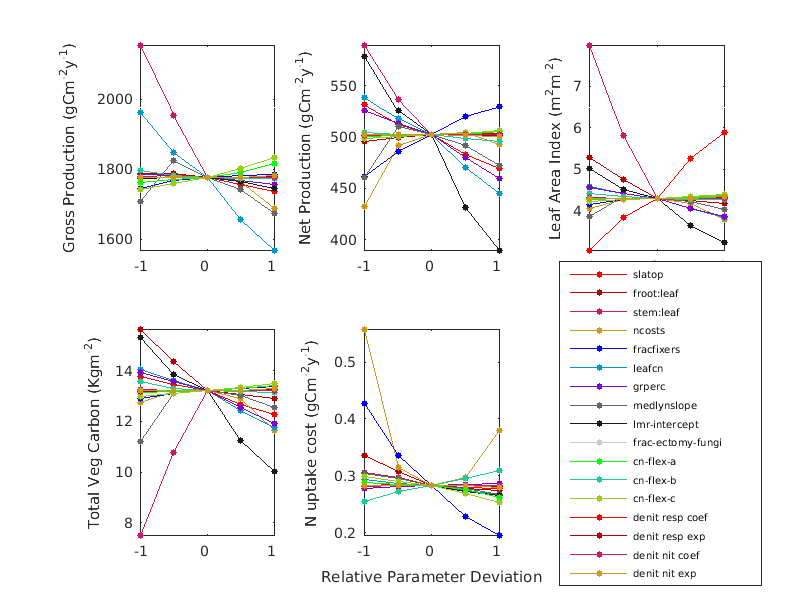
\includegraphics[width=35pc]{matlab/figures/frac_deviation_CO2_response_1CLM5_BCI__y1.png}
     \caption{Response to Nitrogen Deposition}
     \label{BCI CO2 response Parameter Sensitivity}
  \end{figure}
  
  

  
\end{document}